%\chapter*{Введение}
%\addcontentsline{toc}{chapter}{Введение}

\newpage
\begin{center}
\textbf{ГЛАВА 2}\\
\textbf{ВЛИЯНИЕ ДАЛЬНОДЕЙСТВИЯ ПРИТЯЖЕНИЯ НА ФАЗОВЫЕ ДИАГРАММЫ}
\end{center}
\refstepcounter{chapter}


% \section*{}
\addcontentsline{toc}{chapter}{ГЛАВА 2. Влияние дальнодействия притяжения на фазовые диаграммы}

\section{Метод построения фазовых диаграмм с помощью разбиения на ячейки вороного}\label{C2_1}

Метод исследования многочастичных систем с помощью диаграмм Вороного, рассмотренный в статье \cite{Ovcharov2017}, основан на триангуляции Делоне и разбиении систем частиц на ячейки Вороного. Данный метод позволяет разбить систему на ячейки, по статистике которых можно судить о термодинамический параметрах данной системы, и фазовом составе.

Построив гистограмму Вороного для множества точек, каждой точке можно сопоставить ряд параметров:
\begin{itemize}
\item Площадь и плотность.
\item Число соседей (далее будет использован термин \textbf{соседняя частица}).
\item Параметр порядка и т.д.
\end{itemize}

Под плотностью частицы имеется ввиду величина, обратная площади ячейки вороного, которой эта частица принадлежит:
\begin{equation}
\rho_i = 1 / S_i,
\label{eqRho}
\end{equation}
где $\rho_i$ - плотность соответствующей частицы, $S_i$ - ее площадь, определяема как площадь соответствующей ячейки.

Под \textbf{соседней частицей}, понимается частица, с которой имеется общее ребро у ячеек.

\begin{figure}[h]
\begin{center}
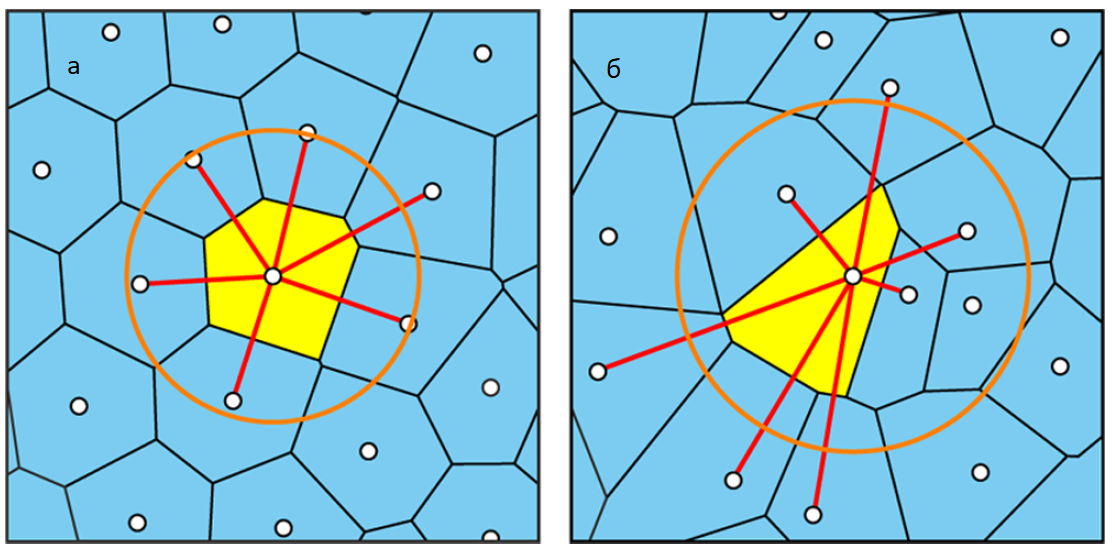
\includegraphics[width=0.7\textwidth]{rgcell}
\caption{Пример разбиения на ячейки Вороного в конденсированном кластере (а) и газе (б). Частицы представлены белыми точками, а ячейки, соответствующие рассматриваемым частицам ячейки раскрашены в желтый цвет. Радиус окружностей соответствует среднему расстоянию между частицей и ее соседями.}
\label{risFlucMed}
\end{center}
\end{figure}

На рисунке \ref{risFlucMed} показана часть $2D$ - системы, полученной с использованием МД-моделирования потенциала Леннарда-Джонса (LJ12-6) при плотности системы $\rho_0 = 0.4$.
Сравнивая ячейки Вороного в конденсированной среде и газе, можно заметить, что конденсированное состояние отличается меньшей площадью частиц, вследствие чего, частицы конденсата обладают большей плотностью, и соответственно, расположение частиц сильно ограниченно в пространстве, что ведет к более упорядоченной структуре и более правильной форме ячеек Вороного.

Это дает возможность ввести некоторую величину, которая будет показывать отклонение ячейки от правильной формы:
\begin{equation}
	R_{0i} = \sqrt{\frac{\pi}{2 S_i N_{ni}^2} \sum\limits_{i<k}^{N_{ni}} (r_{ij} - r_{ik})^2}, r_{ij} = |r_i - r_j|,
\end{equation}
где $S_i$ - площадь рассматриваемой частицы, $N_{ni}$ - количество соседей частицы, $r_{ij}$ - расстояние от рассматриваемой частицы до соседней.
Для уменьшения сильных колебаний величины $R_{0i}$, она усредняется по соседним частицам:
\begin{equation}\label{eqIrreg}
R_i = \frac{1}{N_{ni} + 1} \left( R_{0i} + \sum\limits_{j=1}^{N_{ni}} R_{0j} \right),
\end{equation}

Данная величина позволяет оценить расстояния между соседними частицами, и нормировать их на площадь ячеек.
Далее она будет называться \textbf{параметром иррегулярности $R$}.

\begin{figure}[h]
\begin{center}
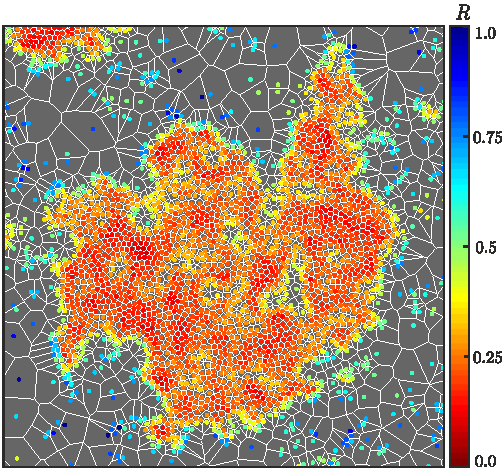
\includegraphics[width=0.7\textwidth]{MPI-Figure1}
\caption{Пример конденсированного кластера в системе с потенциалом Леннарда-Джонса. Ячейки вороного раскрашены в белый цвет, частицы раскрашены по величине параметра иррегулярности $R$.}
\label{risIrreg}
\end{center}
\end{figure}

На рисунке \ref{risIrreg} представлен конденсированный кластер, частицы которого раскрашены в соответствии с параметром иррегулярности. Чем он меньше, тем более упорядочена система. В идеальном кристалле данный параметр равен нулю.

Поскольку параметр $R$ мал для частиц принадлежащих кластерам конденсата, мы можем использовать следующее неравенство для их определения:
\begin{equation}
R < R_t,
\end{equation}
где $R_t$ - порог параметра иррегулярности, ниже которого можно считать частицу конденсатом.

\begin{figure}[h]
\begin{center}
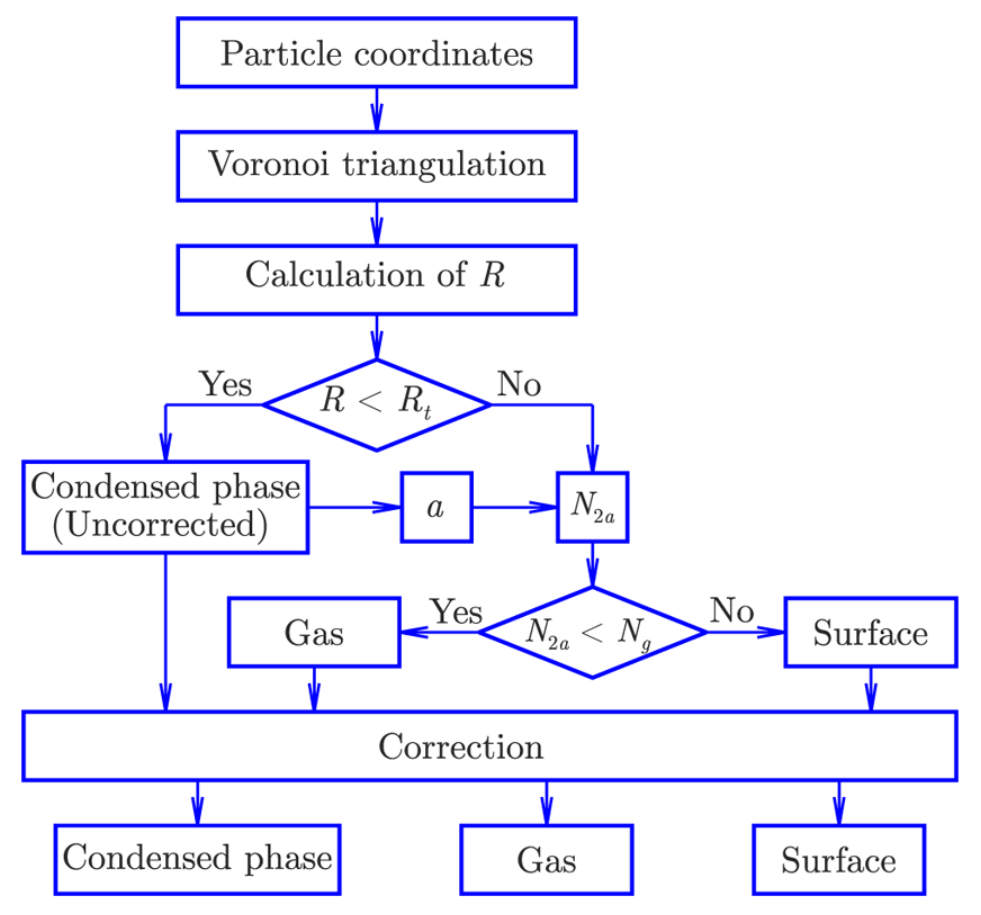
\includegraphics[width=0.5\textwidth]{shem_class}
\caption{Полная схема классификации частиц в системе.}
\label{risShemClass}
\end{center}
\end{figure}

Полная схема классификации частиц в системе, которая использует только координаты, представлена на рисунке \ref{risShemClass},
где $a$ - среднее расстояние между частицами; $N_g$ - некоторое пороговое значение для газовых частиц, находящихся на расстоянии $2a$ от выбранной частицы; $N_{2a}$ - число частиц, находящихся на расстоянии менее $2a$ от выбранной частицы. Если выполняется условие $N_{2a} < N_{g}$, то частица распознается как газ.
В данной работе константы приняты равными $R = 0.5, N_g = 5$.

По причине больший флуктуаций величины $R$, кроме обрезки по параметру $R_t$ и дополнительных условий, требуется корректировка фаз.

Корректировка фаз включает в себя следующие условия:
\begin{itemize}
\item частица конденсата, не имеющая среди своих соседей частиц того же типа, является поверхностью.
\item частица конденсата, которая имеет среди соседних частиц, газовую частицу, является поверхностью.
\item газовая частица, не имеющая соседних частиц того же класса,  является поверхностью.
\item частица поверхности, все соседи которой принадлежат к классу "конденсат" или "газ", так же принадлежат к этому классу.
\end{itemize}
Система частиц прогоняется через эти условия несколько раз. Было установлено, что пяти раз достаточно, для приемлемого результата классификации.

\begin{figure}[h]
\begin{center}
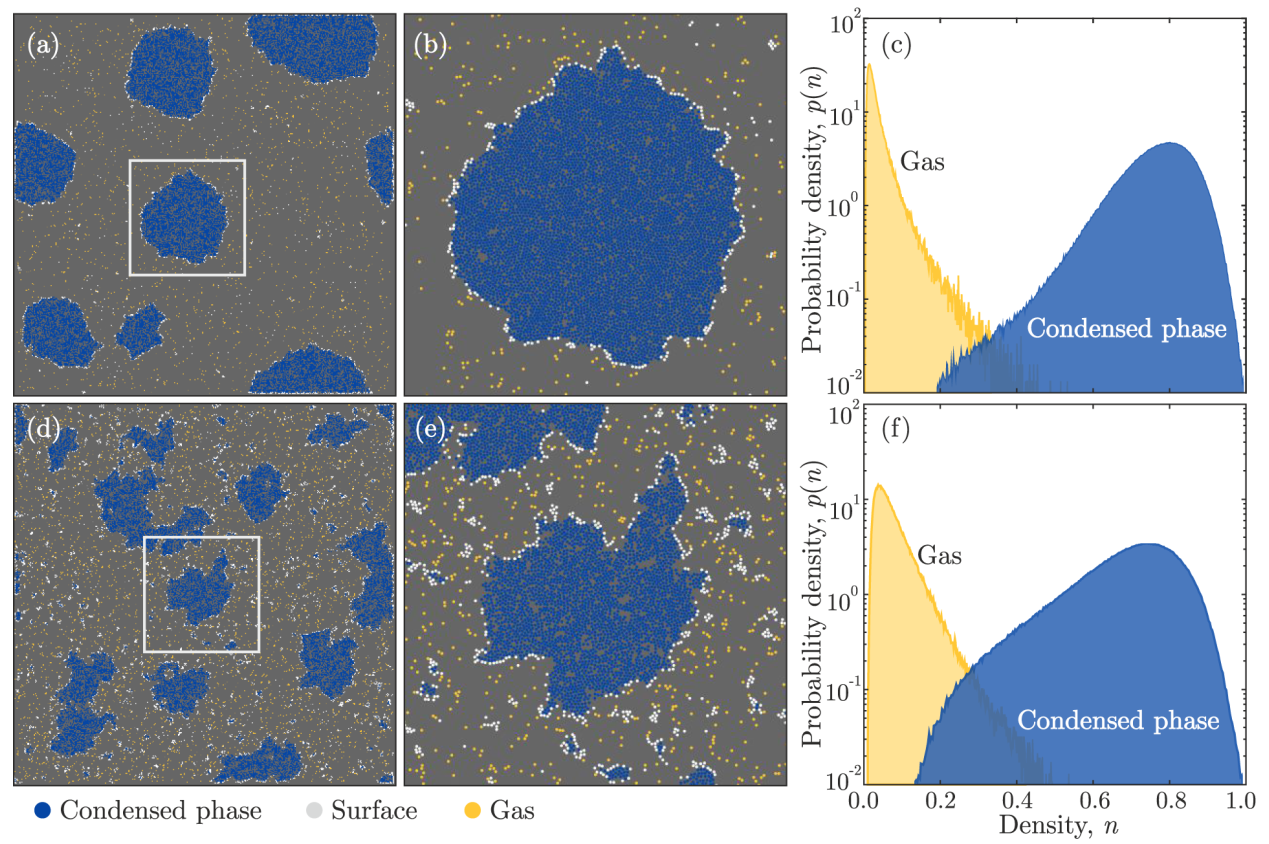
\includegraphics[width=0.8\textwidth]{articlePhaseAndDensity}
\caption{Слева - результат работы алгоритма, представленного на рисунке \ref{risShemClass}. Частицы разделены на 3 класса различными цветами: конденсат - синий, поверхность - белый, газ - желтый. Справа - плотность вероятности нахождения частицы газа и конденсата с данной плотностью.}
\label{risClassification}
\end{center}
\end{figure}

На рисунке \ref{risClassification} представлен результат классификации частиц данным методом в системе описанной выше.
Однако у данного алгоритма есть ряд недостатков. Так например возможны случаи распознавания пустот с газом внутри конденсированного кластера, как его часть, а также наблюдаются крупные скопления частиц поверхности, внутри который нет частиц, распознанных как конденсат.

После классификации всех частиц в системе на всех кадрах моделирования и расчета их плотностей по формуле \ref{eqRho}, возможно рассчитать мат. ожидание плотности конденсированных частиц и газа по-отдельности при данной температуре.
Повторив эти вычисления при различных температурах, можно построить фазовую диаграмму в координатах $\rho, T$.

Однако такой расчет плотности корректно работает только для конденсированных частиц, так как флуктуации размеров ячеек у конденсата невелики, и на их размер не оказывают влияния частицы газа и поверхности. На площадь же газовых частиц существенный эффект оказывают частицы поверхности, которые занимают сопоставимый с ними объем и тем самым увеличивают их плотность. Данная особенность является дефектом этого метода.

В рамках данной работы был существенно переработан алгоритм корректировки фаз, который помимо условий представленных в оригинальной работе включает дополнительные условия:
\begin{itemize}
\item частица поверхности, не имеющая среди соседей частиц газа, является конденсатом.
\item поверхностная частица, не имеющая среди соседей частиц конденсата, является газом.
\item частицы конденсата, плотность которых сопоставима с плотностью поверхностных частиц, являются поверхностью. Данная проверка делается дважды (перед всеми остальными и после).
\item частица конденсата, которая имеет меньше 3 соседних частиц, так же принадлежащих к конденсату, является поверхностью.
\end{itemize}
Эти условия позволяют отделить крупные пустоты внутри кристалла от самого кристалла, и определить крупные скопления поверхностных частиц как небольшие кластеры конденсата или газ.

Так же был переработан алгоритм вычисления плотности газа в системе. Она вычисляется косвенно, по формуле:
\begin{equation}
\rho_{gas} = \frac{N_{g}}{S - (N_{b} + N_{c}) / \mathbb{M}\rho_c},
\label{eqGas}
\end{equation}
где $S$ - суммарная площадь всех рассматриваемых кадров, $N_g, N_b, N_c$ - суммарное число частиц газа, поверхности и конденсата соответственно на всех рассматриваемых кадрах моделирования, $\mathbb{M}\rho_c$ - мат. ожидание плотности частиц конденсата на всех рассматриваемых кадрах.

При данном подходе площадь поверхностных частиц считается равной плотности конденсата, что позволяет более объективно вычислять плотность газа в системе, и соответственно более точно определять критические точки веществ, что будет рассмотрено в главе \ref{C2_2}.

\section{Построение фазовых диаграмм для различных потенциалов взаимодействия}\label{C2_2}

В данной работе, для изучения влияния дальнодействия притяжения на фазовые диаграммы, были выбраны системы с потенциалом взаимодействия обобщенного Леннарда - Джонса (уравнение \ref{eqLJ}), с изменяющейся степенью слагаемого, отвечающего за притяжение:
\begin{equation}
U(r) = 4\varepsilon \left[ \left(\frac{\sigma}{r}\right)^{12} - \left(\frac{\sigma}{r}\right)^{m} \right],
\label{eqLJ}
\end{equation}
где $\varepsilon$ - константа, имеющая размерность энергии, $\sigma$ - константа, имеющая размерность длинны, $r$ - расстояние от центра частицы, $m$ - степень слагаемого, отвечающего за притяжение частиц, в данной работе исследуется ее влияние на фазовые диаграммы и параметры переноса. Далее будет использовано обозначение стандартного потенциала Леннарда - Джонса как LJ12-6, где 12 - степень отталкивания, 6 - степень притяжения.

Были проведены моделирования для случаев $m = 3, 4, 5, 6$ в программе LAMMPS, с параметрами, указанными в таблице \ref{tablParam}, где $\Delta T$ - шаг по температуре,  $\rho$ - плотность системы. Во всех численных экспериментах рассматривалась система в $NVT$ ансамбле, состоящая из 3600 частиц. В ходе моделирования было проделано 600000 итераций изменения системы, между которыми было $0.05\tau$ времени, где $\tau$ - безразмерное эффективное время равное единице. В процессе моделирования данные выводились в файл с периодом в 100 итераций расчета, всего таким образом было получено 6000 состояний системы с интервалом в $0.5\tau$, далее эти состояния будут считаться кадрами моделирования. Что бы исключить эффекты, связанные с релаксацией системы, во всех моделированиях, в качестве данных для анализа, были взяты только последние 150 состояний, в которых система уже находится в равновесии.

Все величины, встречающиеся в данной работе далее, являются обезразмеренными на константы моделирования, такие как масса частиц, постоянную Больцмана, $\varepsilon$ и $\sigma$ в уравнении \ref{eqLJ} потенциала, равные единице.

\begin{table}[h]
\begin{center}
\begin{tabular}{| l | l | l | l | l |}
\hline
    & LJ12-3 & LJ12-4 & LJ12-5 & LJ12-6 \\ \hline
$m$   &    3    &     4   &    5    &    6    \\ \hline
$\Delta T$ & 0.03 & 0.03 & 0.02 & 0.02 \\ \hline
$\rho_0$ & 0.28  &  0.4  &  0.4  &  0.4  \\ \hline
\end{tabular}
\end{center}
\caption{Параметры моделирования исследуемых систем. $m$ - степень слагаемого в уравнении \ref{eqLJ}, $\Delta T$ - шаг по температуре,  $\rho_0$ - плотность системы в целом, то есть количество частиц деленное на площадь всей рассматриваемой системы.}
\label{tablParam}
\end{table}

На примере потенциала Леннарда - Джонса (LJ12-6) продемонстрирована работа модифицированного алгоритма распознавания фаз при различной температуре.

\begin{figure}[h]
\begin{center}
\includegraphics[width=0.7\textwidth]{Voronoi}
\caption{Разбиение на ячейки Вороного различной температуре исследуемой в данной работе системы на примере потенциала Леннарда-Джонса.}
\label{risvoronoiExp}
\end{center}
\end{figure}

На рисунке \ref{risvoronoiExp} изображено разбиение системы на ячейки Вороного для различных температур. При $T = 0.36$ система находится в состоянии кристалла, при $T = 0.44$ в жидком. Также на рисунке представлена система, как выяснится далее, в критической точке ($T = 0.52$) и соответствующая максимальным флуктуациям плотности в системе ($T = 0.60$).

\begin{figure}[h]
\begin{center}
\includegraphics[width=0.7\textwidth]{RG}
\caption{Параметр иррегулярности $R$ в исследуемой системе, на примере потенциала взаимодействия Леннарда-Джонса при различной температуре.}
\label{risIregExp}
\end{center}
\end{figure}

\begin{figure}[h]
\begin{center}
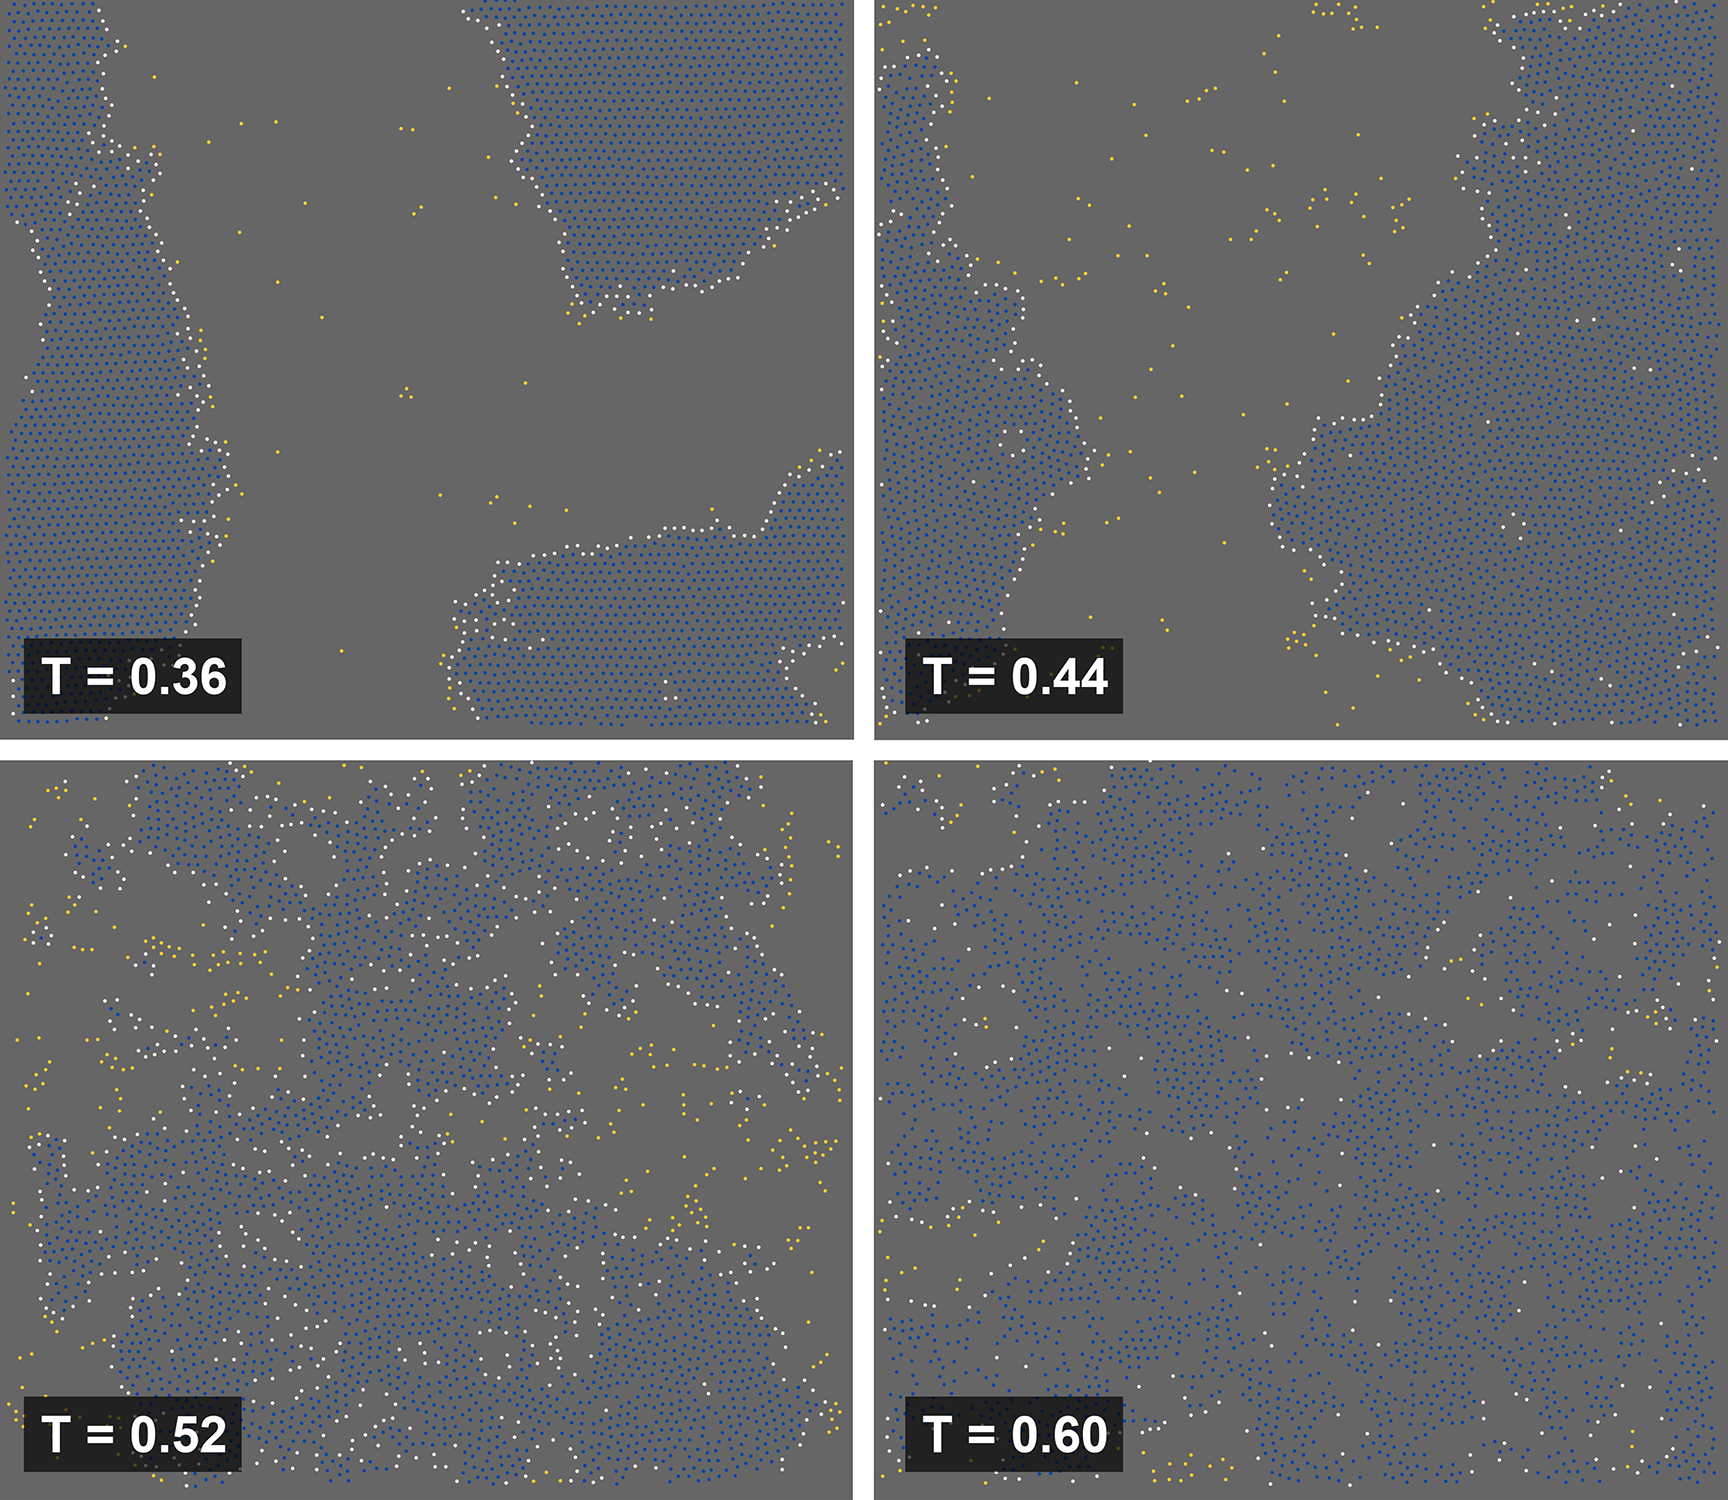
\includegraphics[width=0.7\textwidth]{classification}
\caption{Классификация частиц в исследуемой системы на примере системы c потенциалом взаимодействия Леннарда-Джонса при различной температуре.}
\label{risClassExp}
\end{center}
\end{figure}

После построения диаграммы Вороного проводится расчет параметра иррегулярности, представленного в разделе \ref{C2_1}. Результат расчета параметра изображен на рисунке \ref{risIregExp}. Затем, после корректировки фаз, мы получаем принадлежность каждой частицы к классу конденсата, газа или поверхности (рисунок \ref{risClassExp}).

Как можно увидеть на рисунке \ref{risClassExp}, данный метод лишен недостатков, описанных в главе \ref{C2_1}, связанных с распознаванием фаз.

\begin{figure}[h]
\begin{center}

\begin{minipage}[h]{0.45\linewidth}
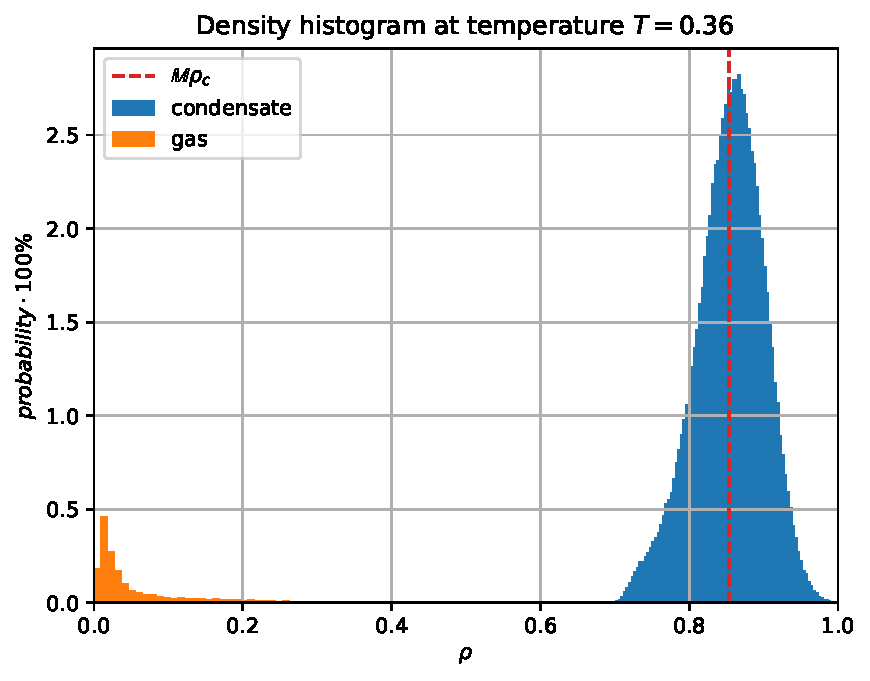
\includegraphics[width=\textwidth, keepaspectratio]{plot_hist_all_0.360}
\end{minipage}
%\hfill
\begin{minipage}[h]{0.45\linewidth}
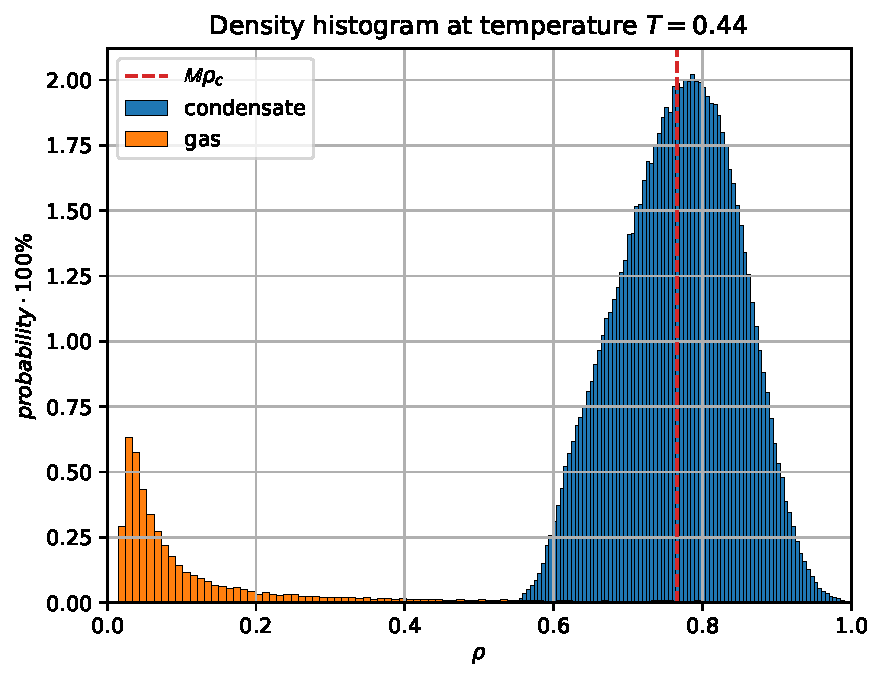
\includegraphics[width=\textwidth, keepaspectratio]{plot_hist_all_0.440}
\end{minipage}

\begin{minipage}[h]{0.45\linewidth}
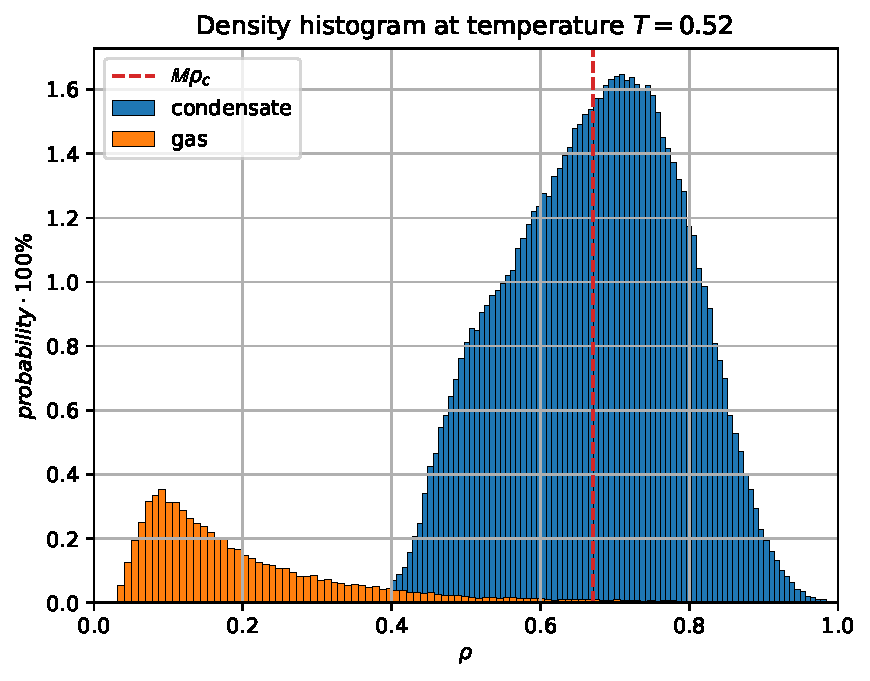
\includegraphics[width=\textwidth, keepaspectratio]{plot_hist_all_0.520}
\end{minipage}
%\hfill
\begin{minipage}[h]{0.45\linewidth}
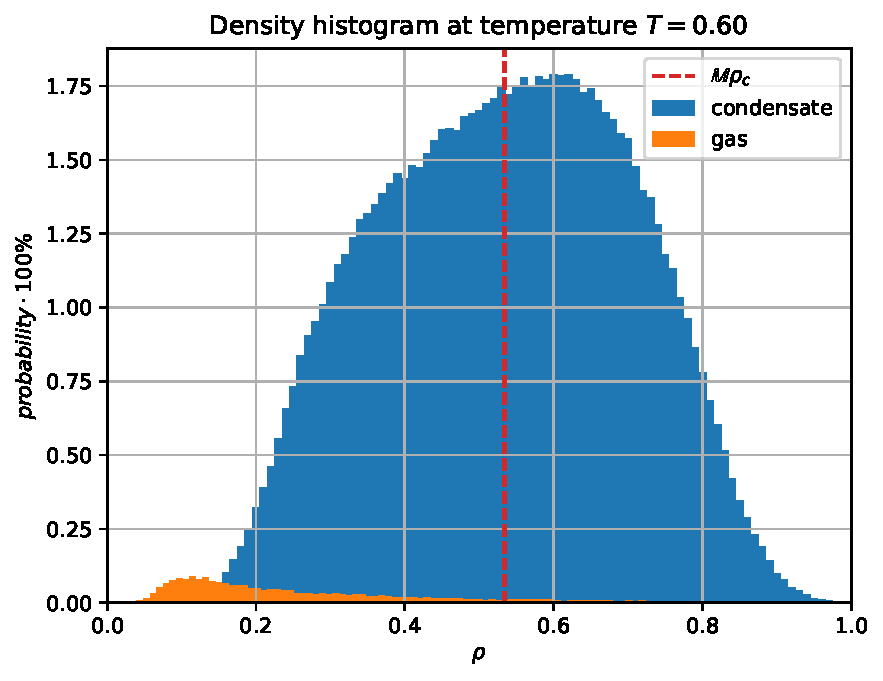
\includegraphics[width=\textwidth, keepaspectratio]{plot_hist_all_0.600}
\end{minipage}
\caption{Распределение плотностей частиц конденсата и газа при различных температурах. Синим цветом обозначен конденсат, оранжевым  - газ.}
\label{risRhoM}
\end{center}
\end{figure}

После классификации частиц, можно приступать к определению мат. ожидания плотности газа и конденсата. На рисунке \ref{risRhoM} изображена график вероятности найти частицу в данной фазе с данной плотностью. Через значение плотности конденсата, указанное на рисунке красной пунктирной линией, можно по формуле \ref{eqGas} найти плотность газа в системе, и повторяя данную процедуру при различной температуре и значениях степени $m$, можно получить фазовые диаграммы для систем с различными потенциалами взаимодействия. Результаты построения фазовых диаграмм для исследуемых потенциалов изображены на рисунке \ref{risPhaseDiagrammExp}.

\begin{figure}[h]
\begin{center}
\begin{minipage}[h]{0.45\linewidth}
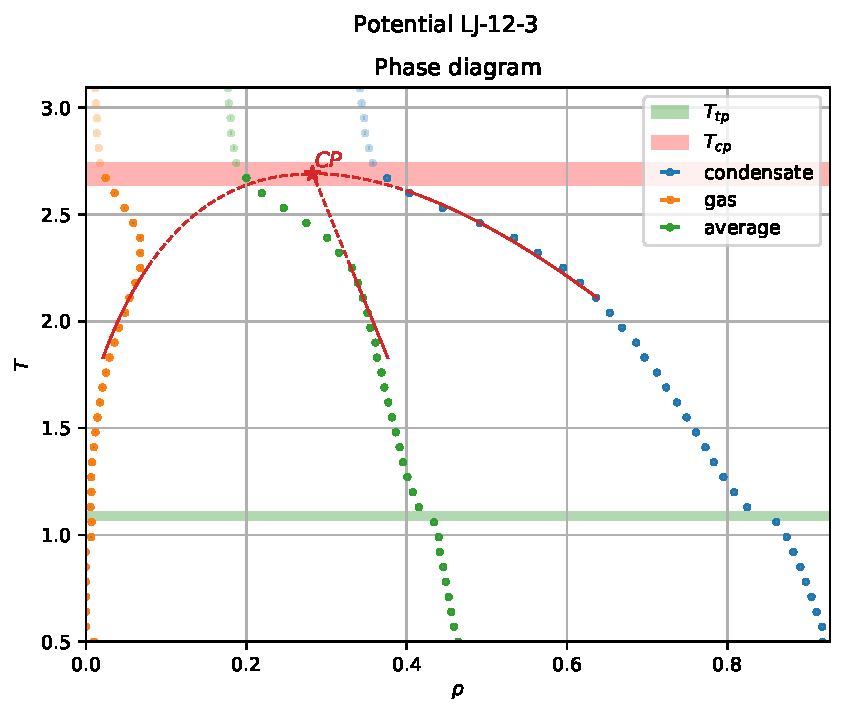
\includegraphics[width=\textwidth, keepaspectratio]{plot_phase_diagram_Potential LJ-12-3_1}
\end{minipage}
%\hfill
\begin{minipage}[h]{0.45\linewidth}
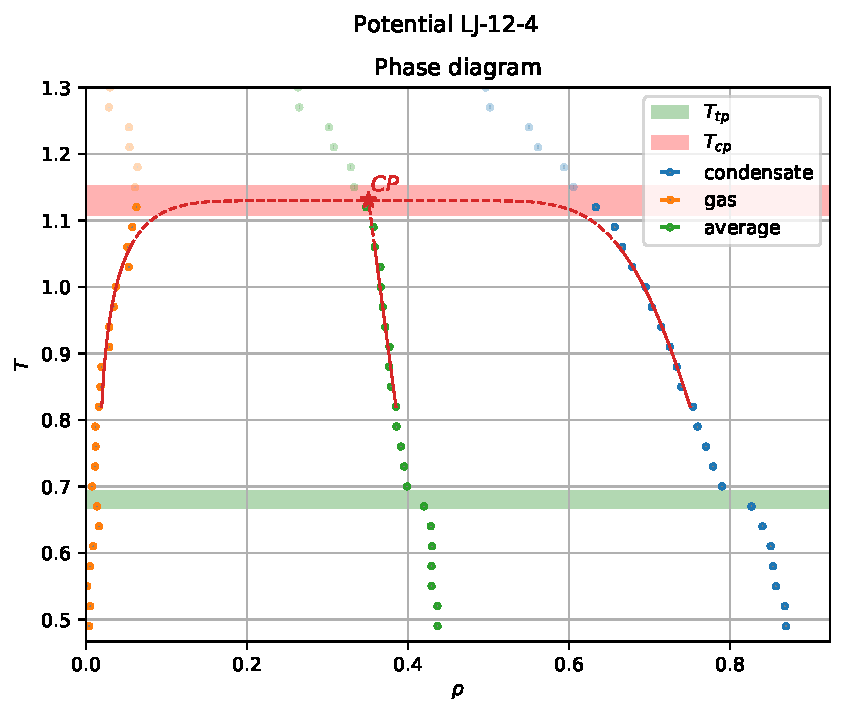
\includegraphics[width=\textwidth, keepaspectratio]{plot_phase_diagram_Potential LJ-12-4_1}
\end{minipage}

\begin{minipage}[h]{0.45\linewidth}
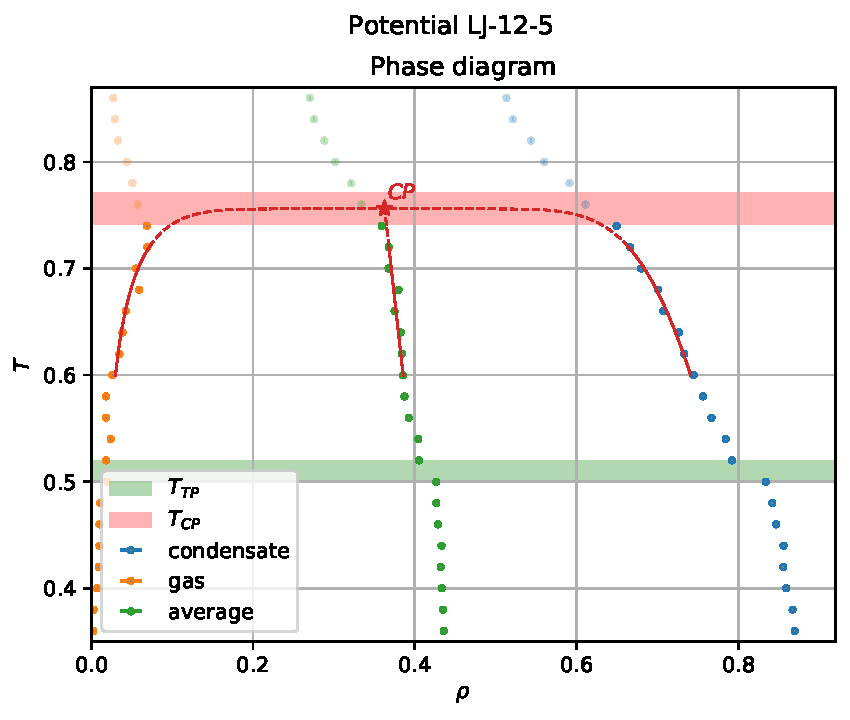
\includegraphics[width=\textwidth, keepaspectratio]{plot_phase_diagram_Potential LJ-12-5_1}
\end{minipage}
%\hfill
\begin{minipage}[h]{0.45\linewidth}
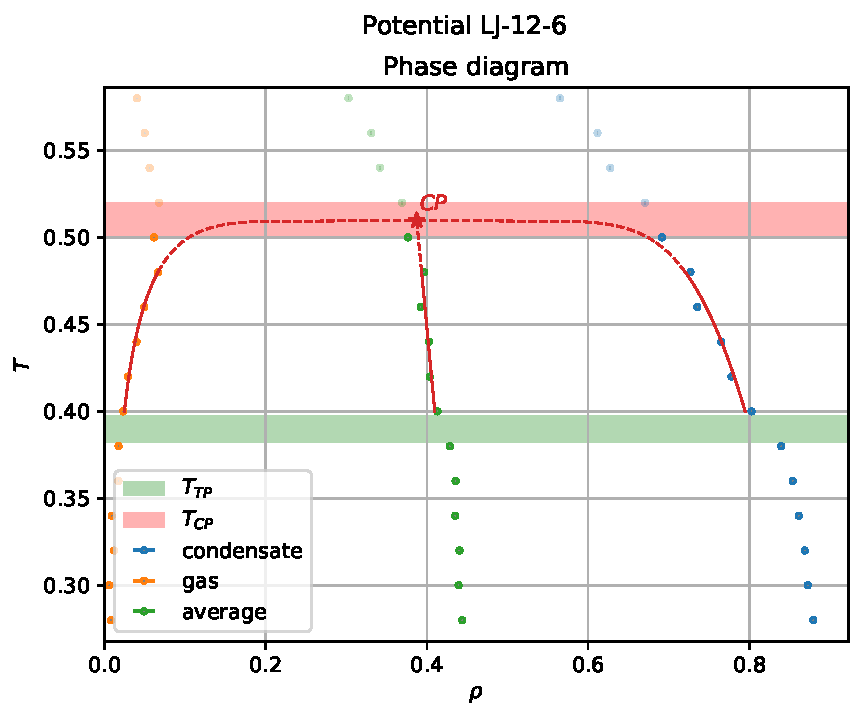
\includegraphics[width=\textwidth, keepaspectratio]{plot_phase_diagram_Potential LJ-12-6_1}
\end{minipage}
\caption{Фазовые диаграммы для систем с исследуемыми потенциалами взаимодействия. Подробности в основном тесте.}
\label{risPhaseDiagrammExp}
\end{center}
\end{figure}

Как известно \cite{fitPhase}, бинодали фазовых диаграммы в координатах $\rho, T$, вблизи критики, описываются следующими уравнениями:
\begin{equation}
\begin{aligned}
\rho_l - \rho_g &\simeq A (T_{CP} - T)^{\beta_c} \\
\frac{\rho_l + \rho_g}{2} &\simeq \rho_{CP} + a(T_{CP} - T)
\end{aligned}
\label{eqFitFhase}
\end{equation}
где $T_{CP}, \rho_{CP}$ - эффективная температура и плотность критической точки, $A, a$ - варьируемые параметры, $\rho_l, \rho_g$ - плотность жидкости и газа соответственно, $\beta_c$ - критический индекс системы.

Согласно источнику \cite{classCrit}, класс универсальности системы зависит от степени притяжения между частицами. Так, система LJ12-3 демонстрирует классическое поведение, для которого критический индекс $\beta_c = 1/2$, для всех остальных потенциалов, рассматриваемых в данной работе, $\beta_c = 1/8$.

Для более точного и удобного определения критической точки с помощью аппроксимации бинодалей, можно записать систему уравнений \ref{eqFitFhase} в следующем виде:
\begin{equation}
f_g(T) = \frac{T-a}{b} - A(T_{CP} - T)^{\beta_c}
\label{eqFitFhaseGas}
\end{equation}
\begin{equation}
f_l(T) = \frac{T-a}{b} + A(T_{CP} - T)^{\beta_c}
\label{eqFitFhaseLicuid}
\end{equation}
\begin{equation}
f_a(T) = \frac{T-a}{b},
\label{eqFitFhaseAverage}
\end{equation}

где уравнение \ref{eqFitFhaseGas} описывает газовую бинодаль, \ref{eqFitFhaseLicuid} - конденсированную, \ref{eqFitFhaseAverage} - их среднее значение, $A, a, b, T_{CP}$ - варьируемые параметры. 

Тогда можно составить функцию невязки, при минимизации которой получить наилучшую аппроксимацию бинодалей и значение критической температуры и плотности.

Условие наилучшей подгонки варьируемых параметров выглядит следующим образом:
\begin{equation}
\min \left(\sum\limits_{k} \left[ f_g(T_{g, k}) - n_{g, k}  \right]^2 + \sum\limits_{k} \left[ f_l(T_{l, k}) - n_{l, k}  \right]^2 + \sum\limits_{k} \left[ f_a(T_{g, k}) - n_{a, k}  \right]^2 \right),
\label{eqFitResidual}
\end{equation}
где суммирование производится по выбранным для аппроксимации точкам, а $n_g, n_l, n_a$ - соответствующие плотности выбранных точек. 

Точки могут быть выбраны не обязательно из одного температурного диапазона, для лучшей точности, чаще всего, выбирается немного различный диапазон. Это связано с некоторыми особенностями данного метода и бесконечным временем релаксации системы вблизи критической точки. Например при приближении к критической точки, из-за выравнивания плотности, существенно падает среднее значение параметра иррегулярности, из-за чего большинство частиц в системе начинает распознаваться как газ. В связи с этим резко начинает падать плотность газа, что не соответствует действительности, поэтому газовая бинодаль аппроксимируется только до момента, пока не меняет свой знак вторая производная плотности по температуре. Данный эффект также влияет и на среднее значение газовой и конденсированной бинодали, поэтому среднее значение также аппроксимируется только до данной температуры.

Конденсированная же ветвь ведет себя более стабильно, и аппроксимация может проводиться по температурам чуть больше, чем для газа и среднего значения, однако в связи с бесконечным временем релаксации системы в критической точке, система не успевает отрелаксировать, и значение плотности конденсата вблизи критики становятся выше реального значения. Поэтому при аппроксимации следует учитывать, что функция, аппроксимирующая конденсированную ветвь бинодали, должна проходить не выше самих точек.

Аппроксимация, проведенная данным методом, изображена на рисунке \ref{risPhaseDiagrammExp}, где красной цельной линией обозначен диапазон температур, точки из которого участвуют в аппроксимации, а красной штриховой - экстраполяция функций \ref{eqFitFhaseGas}, \ref{eqFitFhaseLicuid}, \ref{eqFitFhaseAverage} c найденными на предыдущем шаге подгоночными константами.

Как можно видеть, она довольно хорошо аппроксимирует точки фазовой диаграммы, что позволяет относительно точно определить критическую температуру и плотность системы.
Критические температуры и плотности, определенные данным способом, а так же тройные точки систем приведены в таблице \ref{tablSystemConst}.

\begin{table}[h]
\begin{center}
\begin{tabular}{| l | l | l | l | l |}
\hline
    & $LJ12-3$ & $LJ12-4$ & $LJ12-5$ & $LJ12-6$  \\ \hline
$T_{CP}$    & 2.69  &  1.13   &  0.76  &    0.51   \\ \hline
$T_{TP}$    & 1.09  & 0.68    & 0.51   & 0.40   \\ \hline
$\rho_{CP}$ & 0.28  &  0.35   &  0.36   &  0.39   \\ \hline
\end{tabular}
\end{center}
\caption{Параметры фазовых диаграмм для различных потенциалов взаимодействия. $T_{CP}$ - критическая температура, $\rho_{CP}$ - критическая плотность системы, $T_{TP}$ - температура тройной точки.}
\label{tablSystemConst}
\end{table}

Зная критические точки для потенциалов с различным притяжением, можно установить его роль в фазовой диаграмме вещества. На рисунке \ref{risTcpTtp} изображена зависимость отношения температур критической точки к тройной от степени слагаемого в потенциале \ref{eqLJ}, отвечающего за притяжение. 

\begin{figure}[h]
\begin{center}
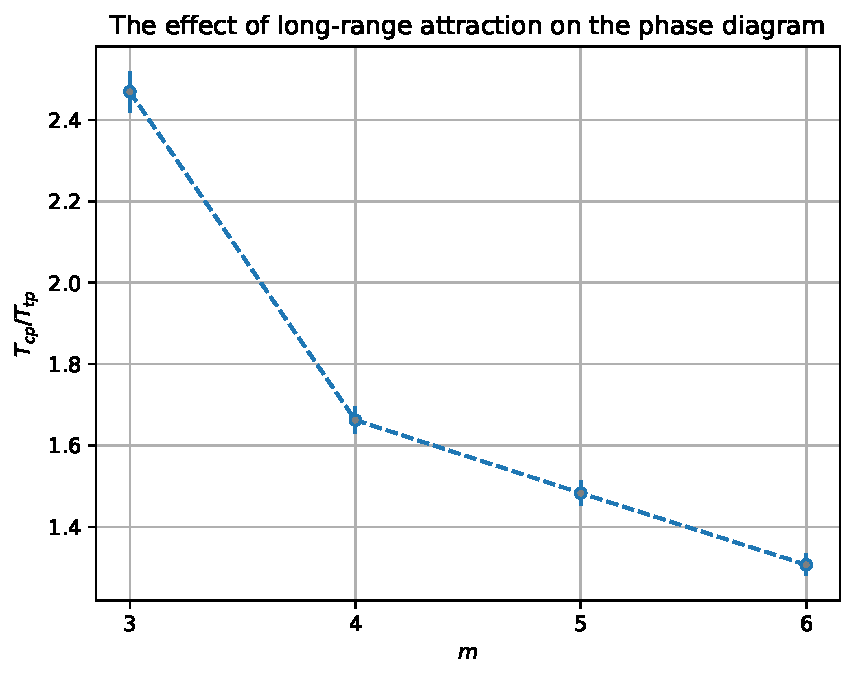
\includegraphics[width=0.7\textwidth]{effect of long-range attraction}
\caption{Отношение температур критической к тройной в зависимости от степени $m$ в уравнении \ref{eqLJ} потенциала.}
\label{risTcpTtp}
\end{center}
\end{figure}

По этим данным можно утверждать, что, скорей всего, функция изображенная на \ref{risTcpTtp} линейна для систем, относящихся к одному классу универсальности.


\section{Анализ гистограмм распределения}\label{C2_3}

Из источника \cite{Landau} следует, что равновесные колебания вблизи среднего значения объема определяются уравнением состояния системы, и соответствующая функция распределения вероятности $p(V)$ равна:
\begin{equation}
p(V) \varpropto \exp\left[ \frac{1}{2T} \left( \frac{\partial P}{\partial V} \right)  \left(V - V_0 \right)^2 \right],
\label{eqPv}
\end{equation}
где $P$ - давление, $V_0$ - максимум распределения объема частиц (площади в $2D$ случае), $V$ - объем (площадь в $2D$ случае) частиц.
Тогда мы можем численно оценить производную $\frac{\partial P}{\partial V}$ и термодинамические величины через нее выражаемые.

Перепишем формулу \ref{eqPv} для колебаний плотности системы, сделав замену $V = 1 / \rho$, и получим следующее уравнение:
\begin{equation}
\begin{aligned}
p(\rho) &\varpropto \exp \left[ - K \left(\rho_{max}- \rho \right)^2 \right] \\
K &= \frac{1}{2T\rho_{max}^2} \left( \frac{\partial P}{\partial \rho} \right)
\end{aligned}
\label{eqFitRho}
\end{equation}
где $\rho_{max}$ - плотность максимума распределения.

\begin{figure}[htbp!]
\begin{center}
\begin{minipage}[h]{0.45\linewidth}
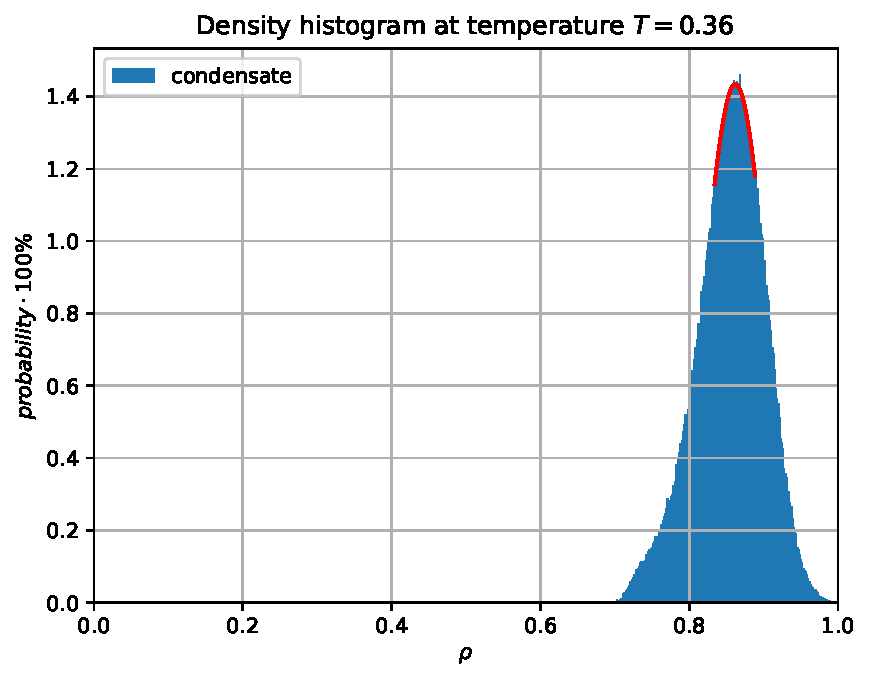
\includegraphics[width=\textwidth, keepaspectratio]{plot_hist_fit_0.360}
\end{minipage}
%\hfill
\begin{minipage}[h]{0.45\linewidth}
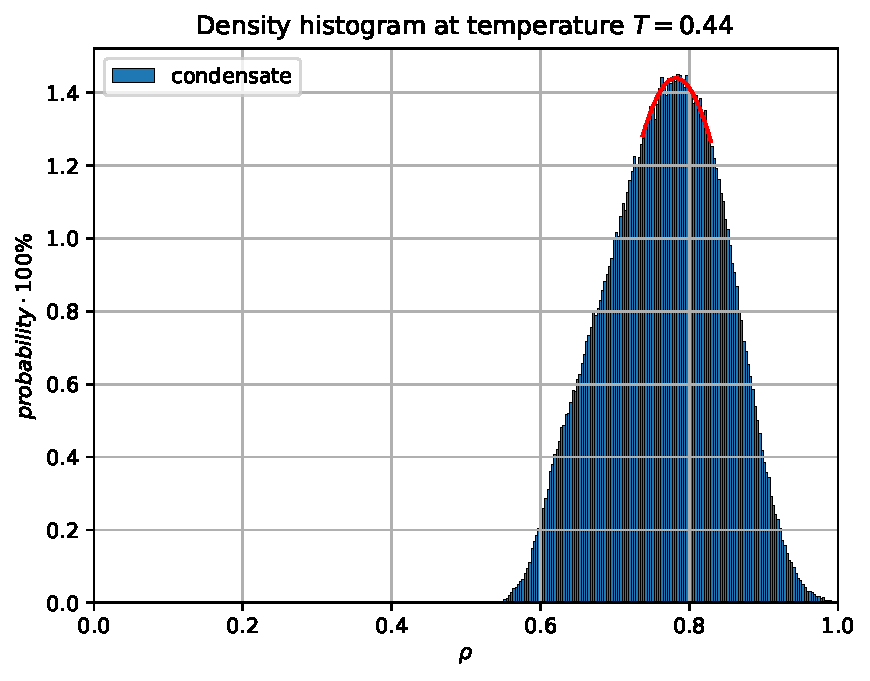
\includegraphics[width=\textwidth, keepaspectratio]{plot_hist_fit_0.440}
\end{minipage}

\begin{minipage}[h]{0.45\linewidth}
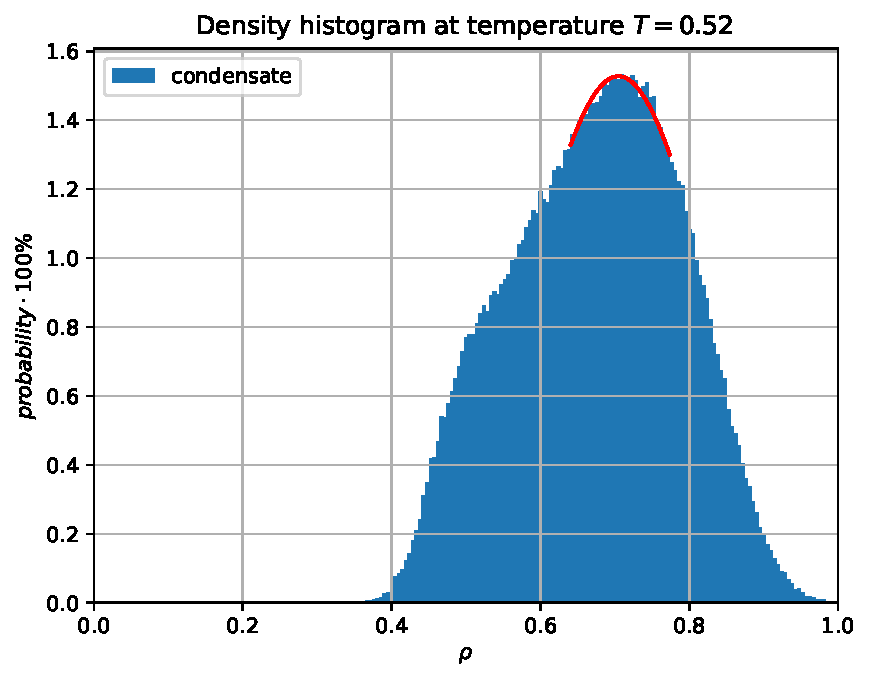
\includegraphics[width=\textwidth, keepaspectratio]{plot_hist_fit_0.520}
\end{minipage}
%\hfill
\begin{minipage}[h]{0.45\linewidth}
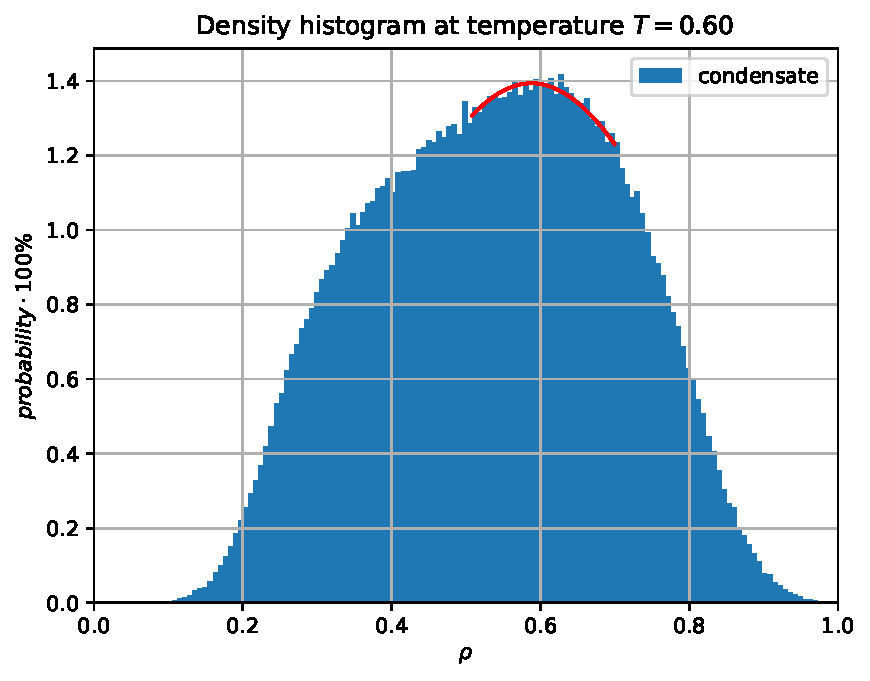
\includegraphics[width=\textwidth, keepaspectratio]{plot_hist_fit_0.600}
\end{minipage}
\caption{Аппроксимация пика распределения плотности при различной температуре.}
\label{risHistFit}
\end{center}
\end{figure}

При аппроксимации пика распределения плотности возникают проблемы с автоматическим определением подгоняемых под уравнение \ref{eqFitRho} точек при различных температурах и величине статистики. Для решения этой проблемы, было решено брать брать точки, отстоящие от пика распределения на $k\sigma$, где $k$ - экспериментально определяемый коэффициент зависящий от формы распределений, для данных систем взятый равным 0.5, $\sigma$ - стандартное отклонение величины $\rho$ от среднего значения.  

Аппроксимируя данным способом верхушку распределения плотностей, для различных температур каждой системы (рисунок \ref{risHistFit}), получаем температурную зависимость коэффициента $K$, стоящего перед квадратичным слагаемом в разложении, представленную на рисунке \ref{risK}.

\begin{figure}[htbp!]
\begin{center}
\begin{minipage}[h]{0.45\linewidth}
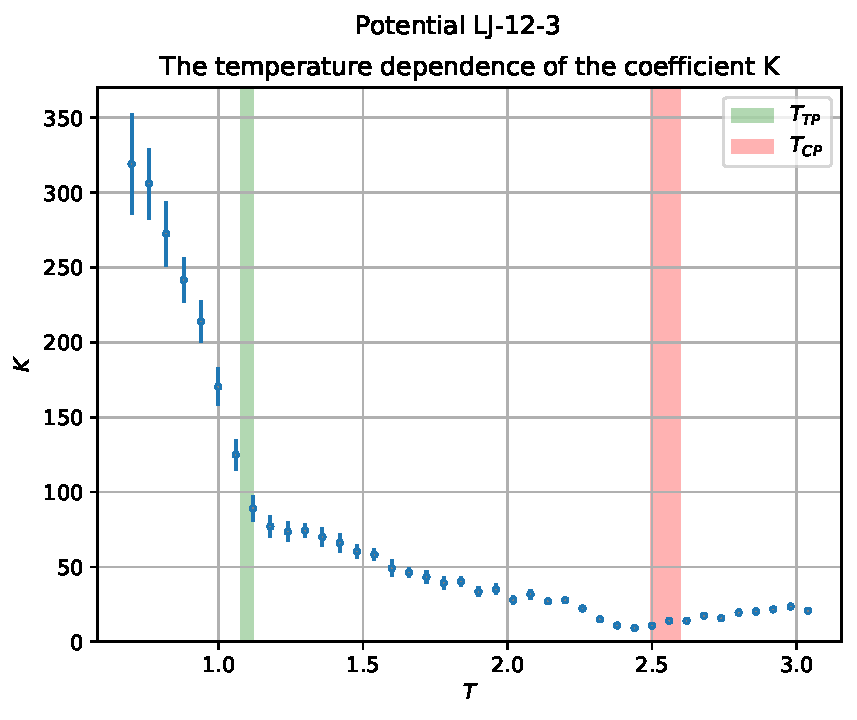
\includegraphics[width=\textwidth, keepaspectratio]{plot_K_Potential LJ-12-3_1}
\end{minipage}
%\hfill
\begin{minipage}[h]{0.45\linewidth}
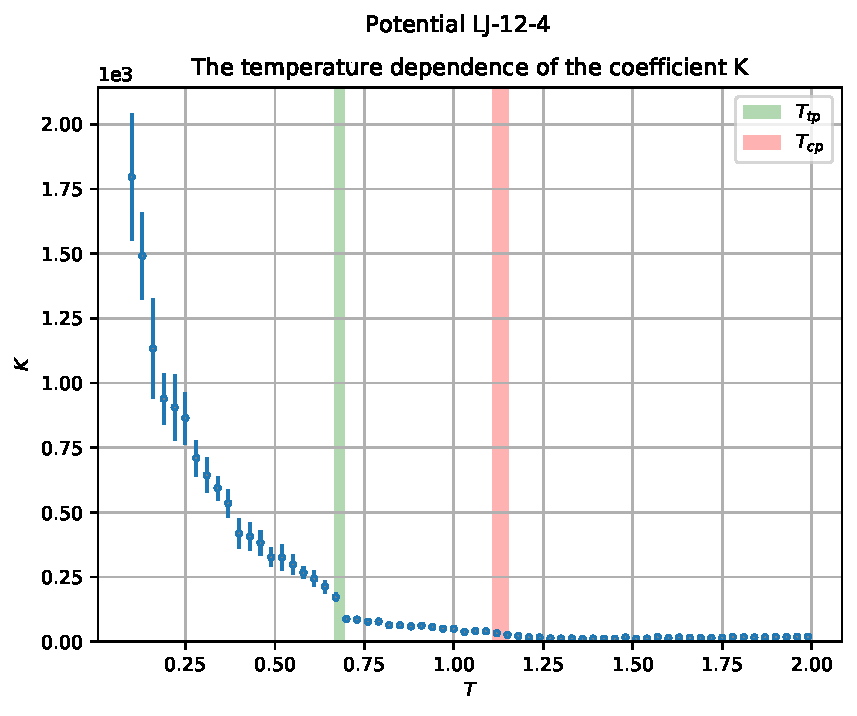
\includegraphics[width=\textwidth, keepaspectratio]{plot_K_Potential LJ-12-4_1}
\end{minipage}

\begin{minipage}[h]{0.45\linewidth}
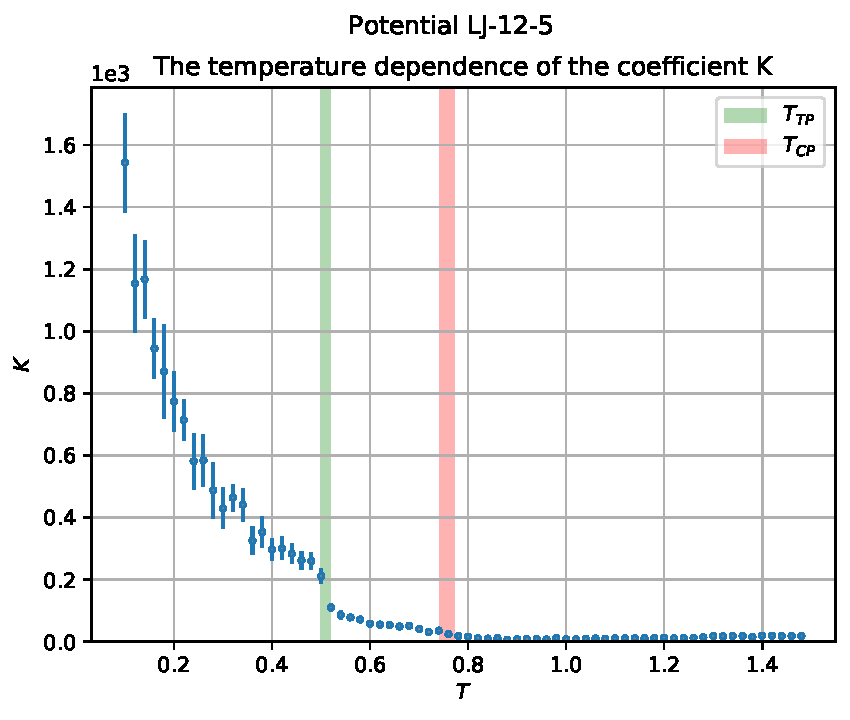
\includegraphics[width=\textwidth, keepaspectratio]{plot_K_Potential LJ-12-5_1}
\end{minipage}
%\hfill
\begin{minipage}[h]{0.45\linewidth}
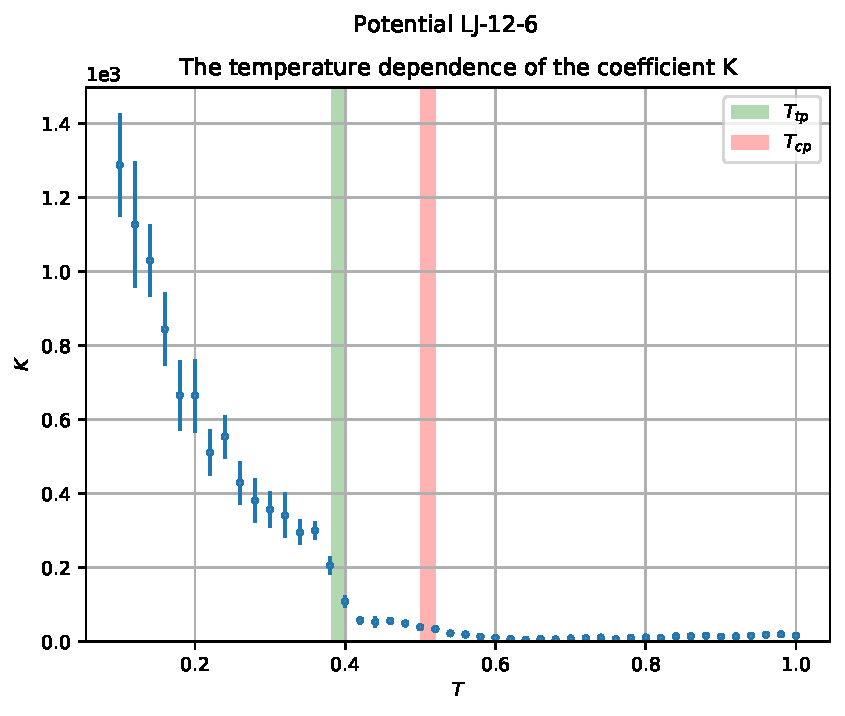
\includegraphics[width=\textwidth, keepaspectratio]{plot_K_Potential LJ-12-6_1}
\end{minipage}
\caption{Температурная зависимость коэффициента $K$.}
\label{risK}
\end{center}
\end{figure}

Через данный коэффициент можно выразить некоторые свойства системы, определяемые производной $\frac{\partial \rho}{\partial P}$, например сжимаемость вещества и адиабатическую скорость звука.

По определению, сжимаемость и адиабатическая скорость звука выражаются следующими формулами:
\begin{equation}
\beta = \frac{1}{\rho_0} \frac{\partial \rho}{\partial P}
\label{eqBetaClassic}
\end{equation}
\begin{equation}
C = \sqrt{\frac{\partial P}{\partial \rho}},
\label{eqCClassic}
\end{equation}
где $\beta$ - сжимаемости, $C$ - скорость звука в веществе.

Выразив данные величины через коэффициент $K$, получим следующие формулы:
\begin{equation}
\beta = \frac{1}{2T\rho_0\rho_{max}^2K}
\label{eqBeta}
\end{equation}
\begin{equation}
C = \rho_{max}\sqrt{2TK}
\label{eqC}
\end{equation}
Проведя вычисления при различных температурах, получаем зависимость сжимаемости и скорости звука в системе, рисунки \ref{risBeta} и \ref{risC}.

\begin{figure}[h]
\begin{center}
\begin{minipage}[h]{0.45\linewidth}
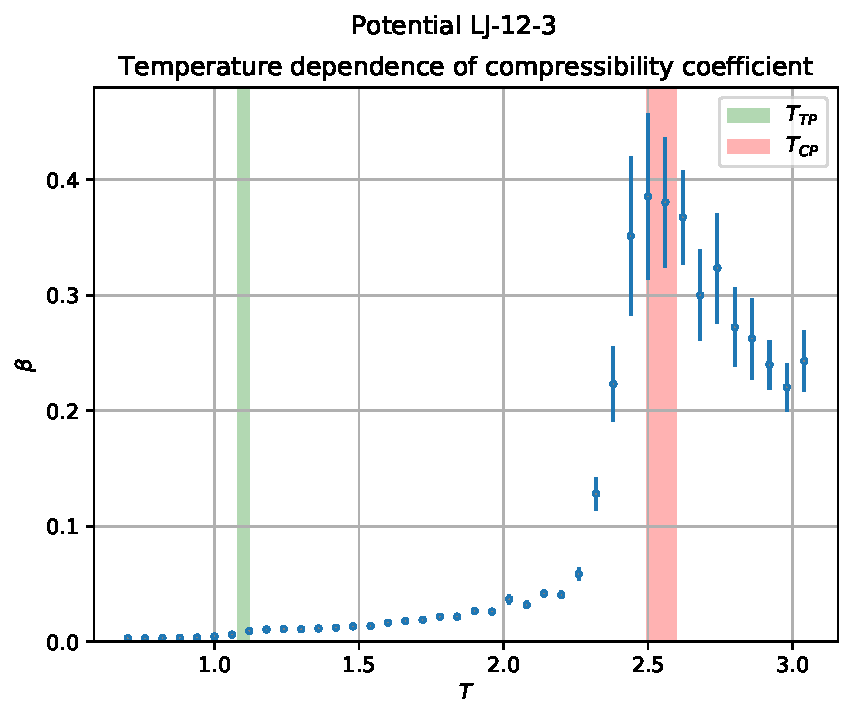
\includegraphics[width=\textwidth, keepaspectratio]{plot_compress_Potential LJ-12-3_1}
\end{minipage}
%\hfill
\begin{minipage}[h]{0.45\linewidth}
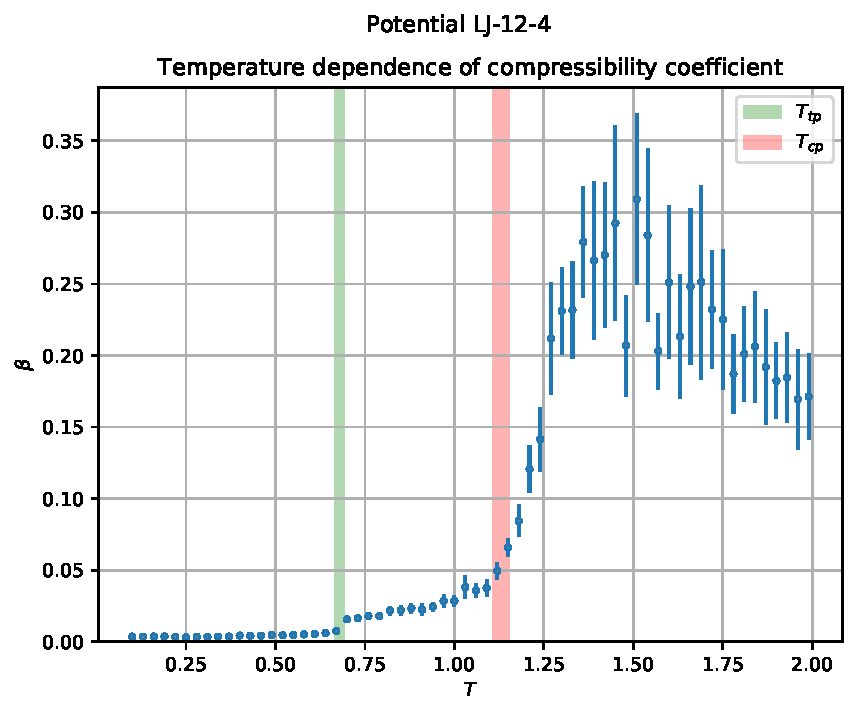
\includegraphics[width=\textwidth, keepaspectratio]{plot_compress_Potential LJ-12-4_1}
\end{minipage}

\begin{minipage}[h]{0.45\linewidth}
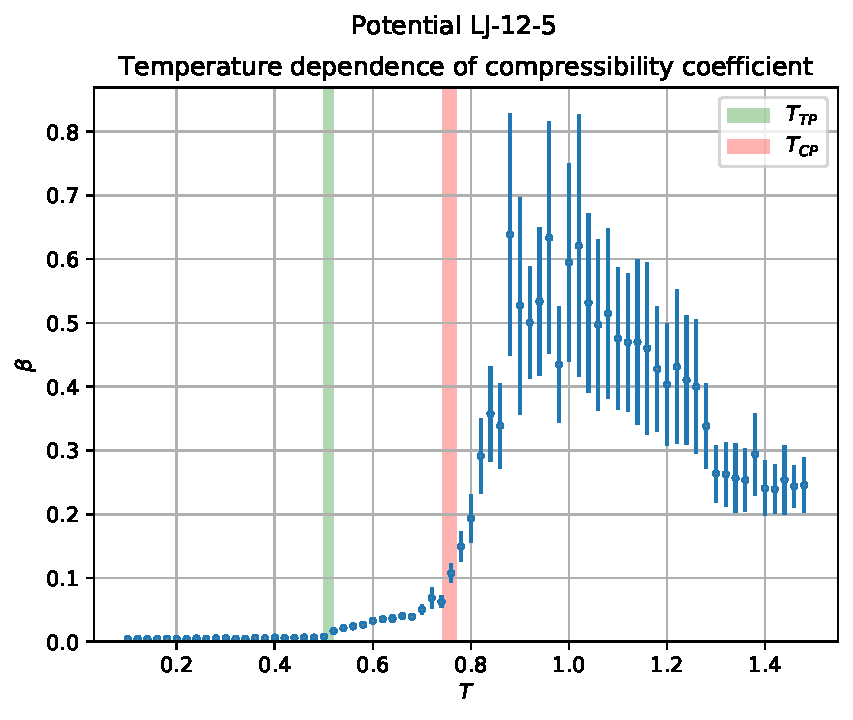
\includegraphics[width=\textwidth, keepaspectratio]{plot_compress_Potential LJ-12-5_1}
\end{minipage}
%\hfill
\begin{minipage}[h]{0.45\linewidth}
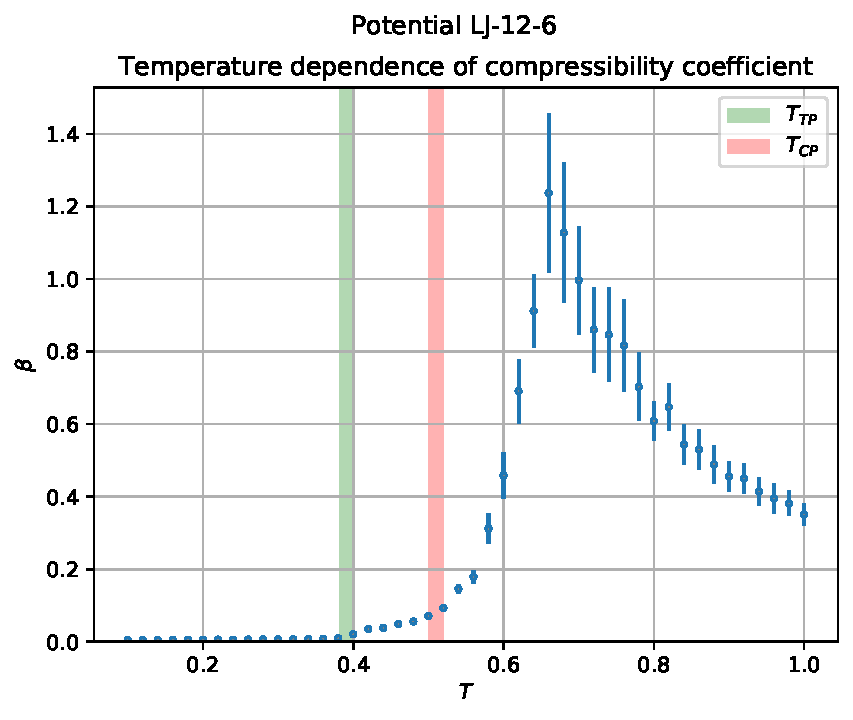
\includegraphics[width=\textwidth, keepaspectratio]{plot_compress_Potential LJ-12-6_1}
\end{minipage}
\caption{Температурная зависимость коэффициента $\beta$ сжимаемости вещества.}
\label{risBeta}
\end{center}
\end{figure}


\begin{figure}[h]
\begin{center}
\begin{minipage}[h]{0.45\linewidth}
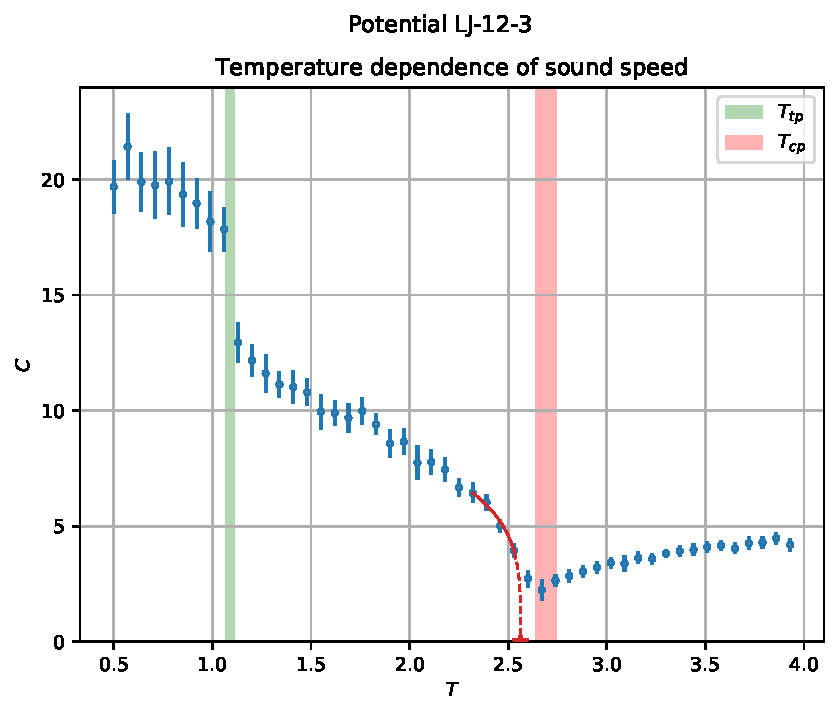
\includegraphics[width=\textwidth, keepaspectratio]{sound_speed_Potential LJ-12-3_1}
\end{minipage}
%\hfill
\begin{minipage}[h]{0.45\linewidth}
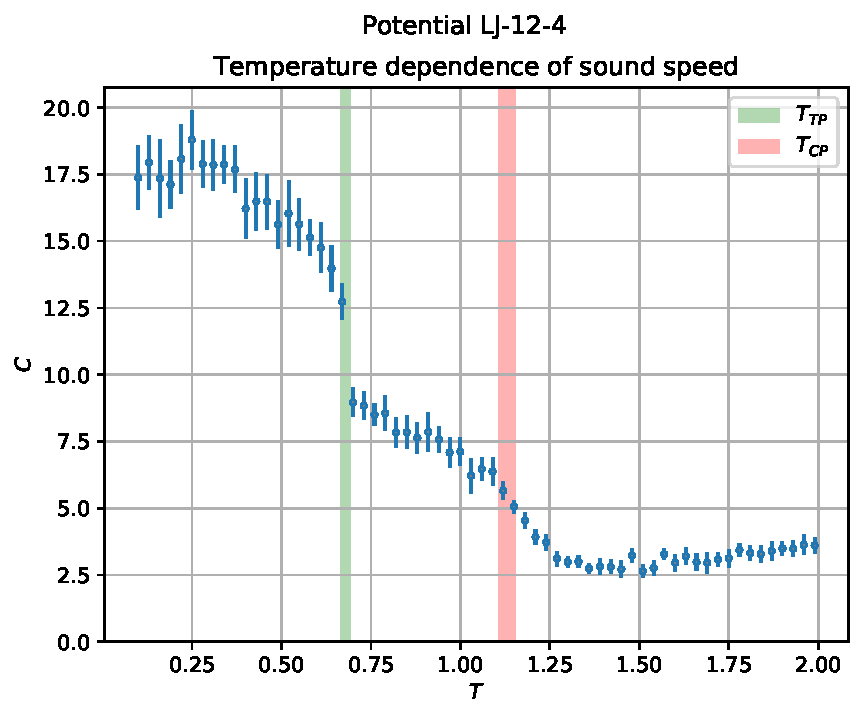
\includegraphics[width=\textwidth, keepaspectratio]{sound_speed_Potential LJ-12-4_1}
\end{minipage}

\begin{minipage}[h]{0.45\linewidth}
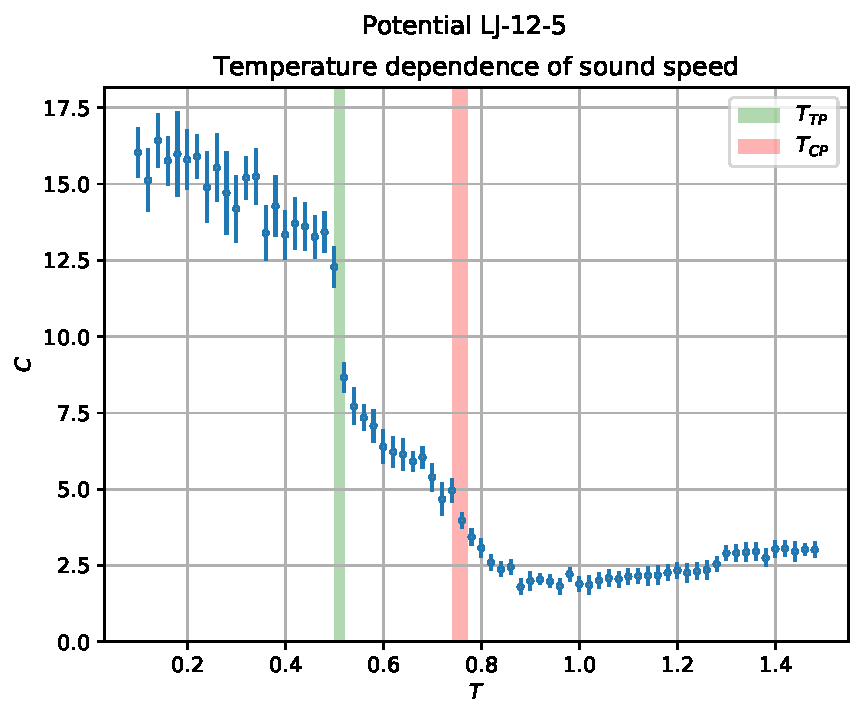
\includegraphics[width=\textwidth, keepaspectratio]{sound_speed_Potential LJ-12-5_1}
\end{minipage}
%\hfill
\begin{minipage}[h]{0.45\linewidth}
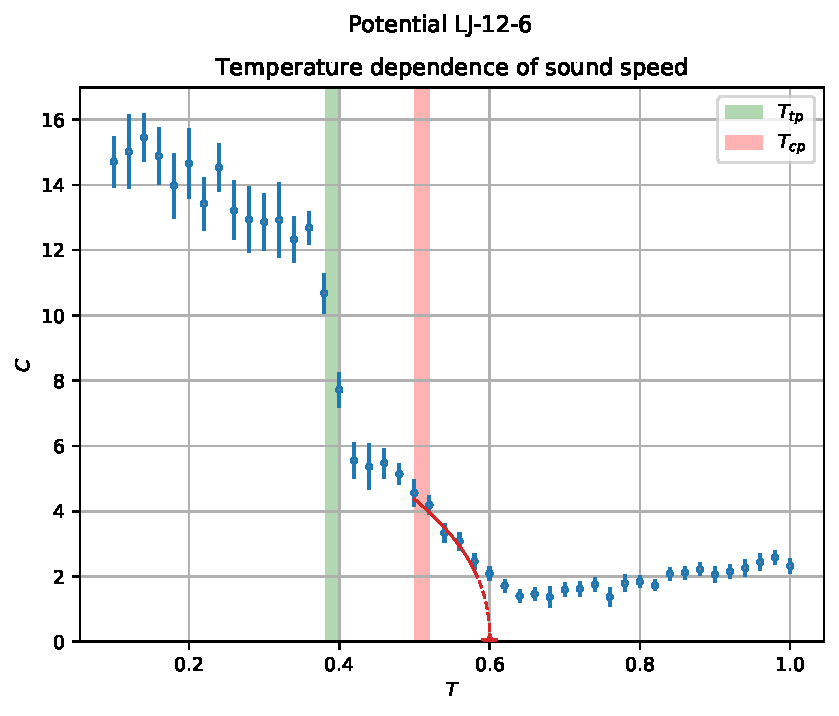
\includegraphics[width=\textwidth, keepaspectratio]{sound_speed_Potential LJ-12-6_1}
\end{minipage}
\caption{Температурная зависимость скорости звука в веществе. Красной сплошной линией обозначена область температуры, точки из которой участвуют в аппроксимации, штриховой линией обозначена экстраполяция скорости звука.}
\label{risC}
\end{center}
\end{figure}

Из источника \cite{soundSpeed} известно, что зависимость скорости звука вблизи критической точки изменяется по закону:
\begin{equation}
    C \sim v(T_{CP} - T)^{(1-\beta_c)/2},
    \label{eqFitC}
\end{equation}
где $v$ - подгоночный коэффициент.

Аппроксимировав данной зависимостью скорость звука (красная линия на рисунке \ref{risC}), можно проверить правильность определения критической точки методом, предложенным в разделе \ref{C2_1}.

Кроме того, интересное поведение проявляют температурные зависимости моментов плотности, изображенные на рисунке \ref{risMu}.

Данные величины вычисляются по следующей формуле:
\begin{equation}
\mu_i = \mathbb{M} \left[ |\rho - \mathbb{M} \rho|^i \right]
\end{equation}
По данной зависимости можно судить о температуре с максимальными флуктуациями плотности системы, так называемой линии Уидома.

\begin{figure}[h]
\begin{center}
\begin{minipage}[h]{0.45\linewidth}
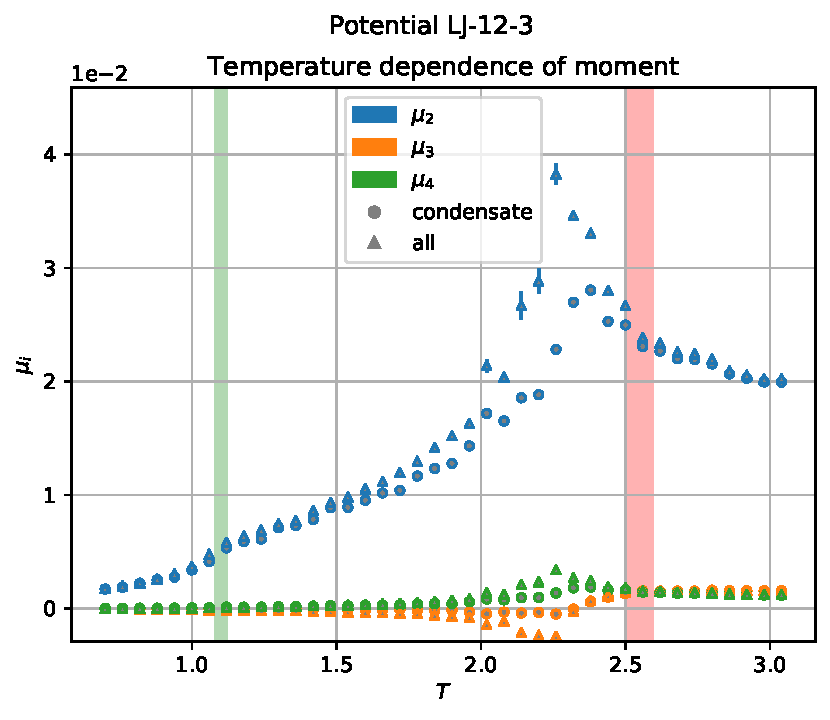
\includegraphics[width=\textwidth, keepaspectratio]{plot_moment_Potential LJ-12-3_1}
\end{minipage}
%\hfill
\begin{minipage}[h]{0.45\linewidth}
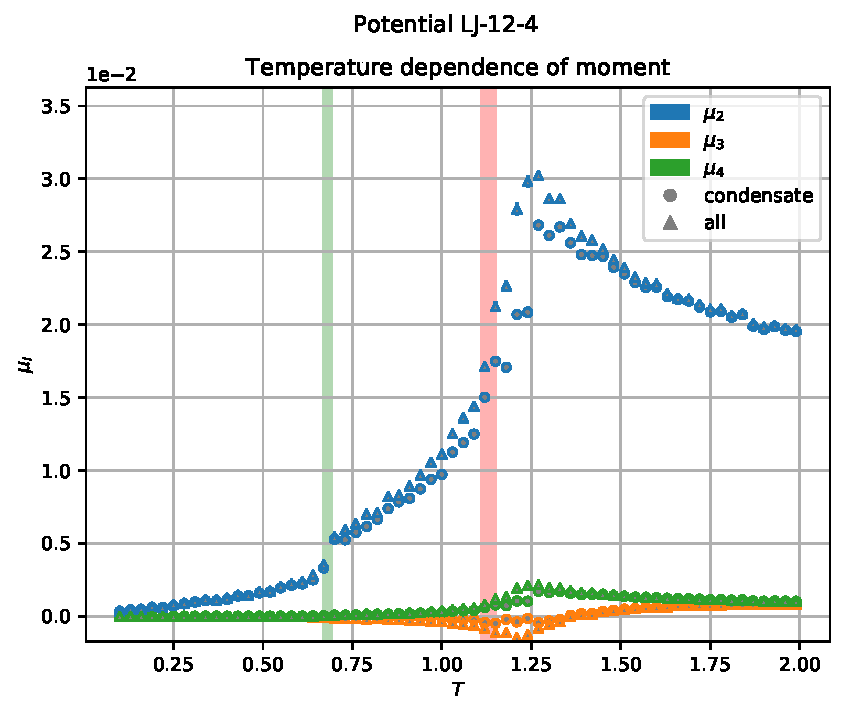
\includegraphics[width=\textwidth, keepaspectratio]{plot_moment_Potential LJ-12-4_1}
\end{minipage}


\begin{minipage}[h]{0.45\linewidth}
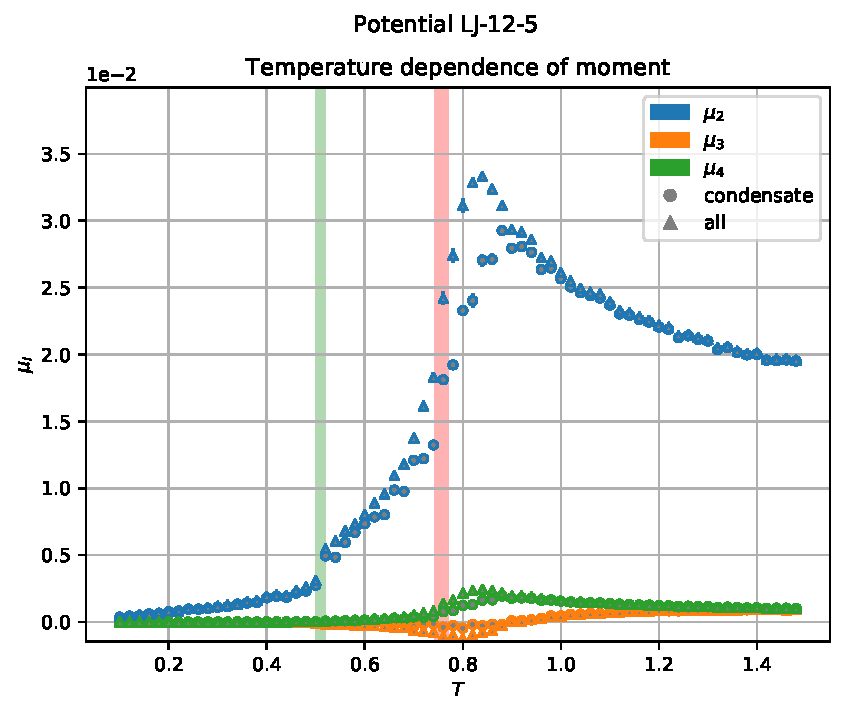
\includegraphics[width=\textwidth, keepaspectratio]{plot_moment_Potential LJ-12-5_1}
\end{minipage}
%\hfill
\begin{minipage}[h]{0.45\linewidth}
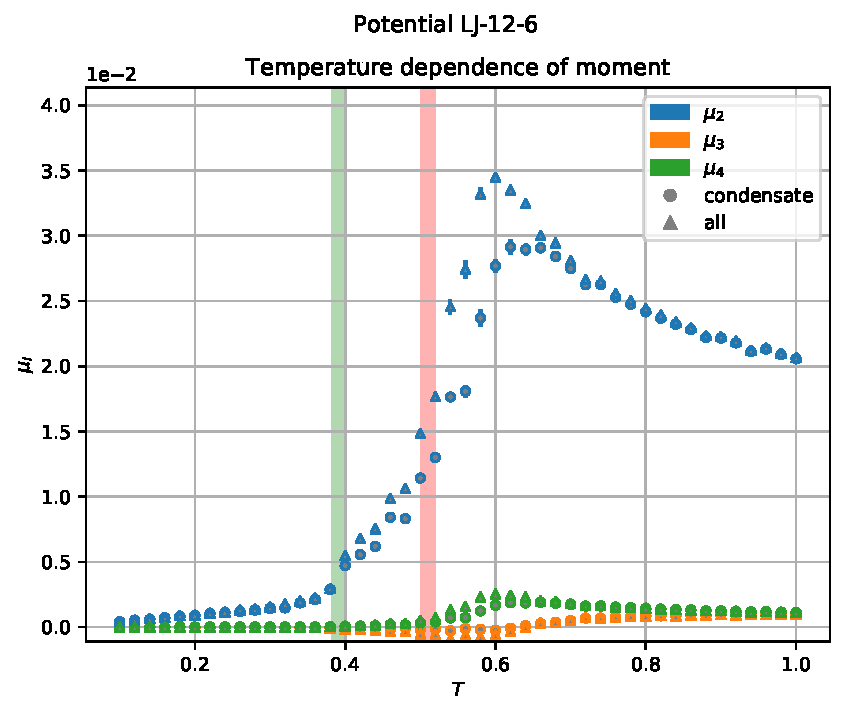
\includegraphics[width=\textwidth, keepaspectratio]{plot_moment_Potential LJ-12-6_1}
\end{minipage}
\caption{Температурная зависимость моментов величины $\mu$.}
\label{risMu}
\end{center}
\end{figure}



\section{Выводы главы}\label{C2_4}

Таким образом, был рассмотрен методы, которые позволяют определить некоторые термодинамические свойтва системы, используя только координаты частиц в системе. Был продемонстрирован метод распознавания фаз, позволяющий классифицировать все частицы в системе как газ, поверхность или конденсат, который был существенно модернизирован в рамках данной работы, и в некоторых случаях позволяет существенно улучшить распознавание фаз.
Также в данной главе был рассмотрен способ получения фазовых диаграмм в координатах $\rho, T$, который основан на вычислении математического ожидания плотности конденсата и косвенного определения плотности газа, что является нововведением для данного метода, позволяющим убрать влияние поверхностных частиц на значения плотности газа. 
Был рассмотрен метод получения значений критической точки, с помощью аппроксимации ветвей бинодали, который удалось автоматизировать с помощью составления функции невязки для произвольных критических коэффициентов.
Кроме этого, в статье был рассмотрен способ вычислений коэффициента сжимаемости и скорости звука в веществе, используя только статистику распределение плотностей в системе. Так же по данной статистике удалось определить температуру наибольших флуктуаций плотности в системе.

Результат работы всех этих методов дает возможность выяснить влияние притяжения в системе на фазовые диаграммы, что позволяет предсказывать поведение систем с тем или иным притяжением взаимодействия.
